\chapter{Design}\label{C:design}

The design of the estimator was in direct correspondence with the system it describes and predicts. With the Bayesian framework, we obtain a belief in order to form an effective estimation. There are several assumptions made to allow the estimator to be simple yet robust for application.


Figure \ref{fig:test_topology} describes the overall computational work-flow of the estimator.


\begin{figure}[h]
    \centering
    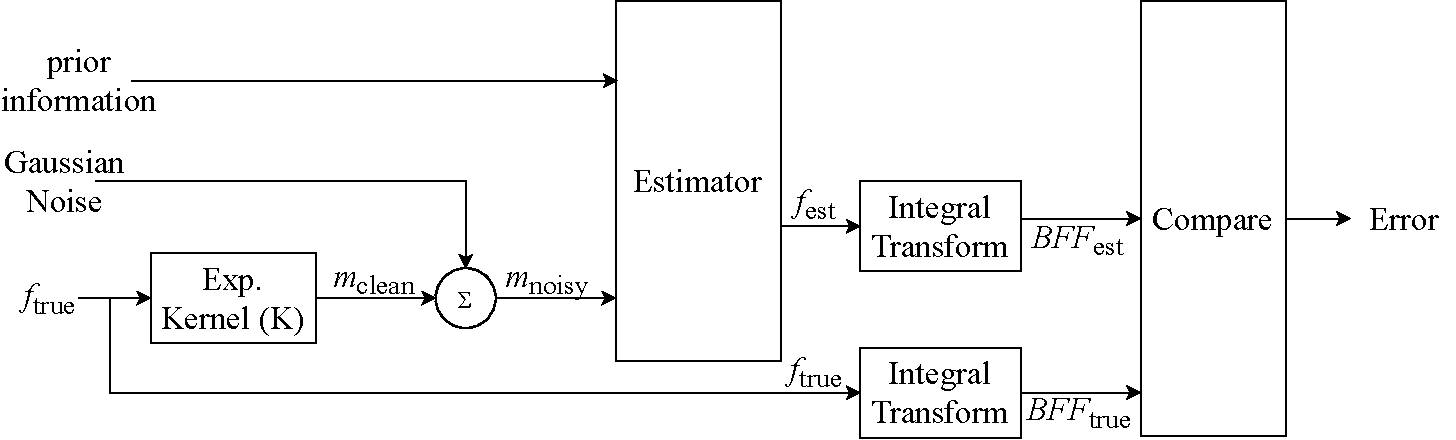
\includegraphics[width=\textwidth]{design/SystemWorkflow489.pdf}
    \caption{The topology of the test architecture of the proposed $BFF$ estimators}
    \label{fig:test_topology}
\end{figure}

\section{The Bayesian Model} \label{section:bayesTechniqueDesign}
There are a series of fundamental assumptions on how NMR T2 relaxation measurements typically behave to support a Bayesian estimation framework. Setting the general constraints that the model may operate on are essential so that it may deliver usable results. Additionally, adapting aspects of models from previous literature into a Bayesian context allows for direct comparability. The topology of the proposed Bayesian framework is detailed in Figure \ref{fig:bayesian_framework}.


\begin{figure}[h]
    \centering
    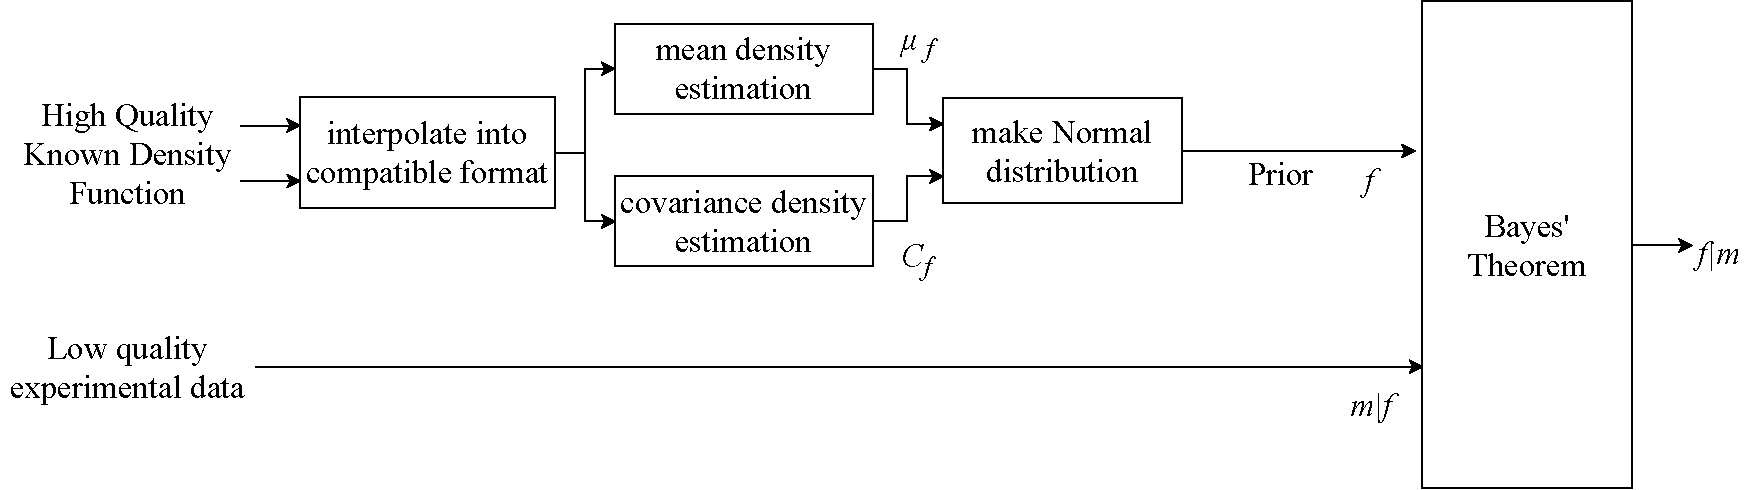
\includegraphics[width=\textwidth]{design/BayesianTechniqueTopology.pdf}
    \caption{Structure of the Bayesian framework of the estimator}
    \label{fig:bayesian_framework}
\end{figure}


\subsection{Modelling the Measurement}
The time domain T2 relaxation measurement, $m$, is the starting point for the Bayesian estimator model. We assume the noise is additive, zero mean, Gaussian and white (i.e., each time domain measurement is independent of each other; the noise from one measurement does not `leak' into the next measurement) This means that the $m$ vector has a diagonal covariance matrix, $C_m$, that describe its uncertainty.


To borrow from the previous literature, we can hypothesise that a measurement is the result of a mapping of the true density function of relaxation times to the time domain by a kernel matrix, $K$. The kernel matrix maps relaxation times to a time domain exponential decay. Therefore, we obtain a measurement vector from a density function that we are trying to find. This results in our the measurement noise distribution:
\begin{equation}
    \label{eq:bayes_measure_given_function}
    m|f \sim \mathcal{N}(Kf, C_m) \text{,   } K \in \mathbb{R}^{N_y \times N_{2}}
    \text{,   } C_m \in \mathbb{R}^{N_y \times N_y} \text{,   } f \in \mathbb{R}^{N_{2}}
\end{equation}
We use this as part of our quotient in the Bayesian framework.  



\subsection{Density Function Model}
The aim of the first stage of the estimator is to obtain the density function of T2 relaxation conditioned on the measurement data. This is the posterior in the Bayesian framework, p$(f|m)$. Obtaining this density function requires finding p$(f)$ and p$(m)$ in the framework as well. 

\subsubsection{Modelling the prior}
The prior is modelled as a multivariate Gaussian. There are two components: a vector of mean magnitudes at different bins of T2 relaxation times, $ \mu_f $; and a covariance matrix of the variance of each density value and cross-correlation between different relaxation bins, $C_f$. This structure allows for a straightforward and tractable framework. This also forms a significant design point of the system detailed in Section \ref{section:makingPrior}.


An important limitation of the Gaussian assumption is that a Gaussian distribution allows for negative relaxation times. Negative values violate the non-negative assumption that is required for the decaying exponential kernel that forms the measurement data.


\subsubsection{Modelling the quotient}

In order to obtain a directly attainable density function estimation, all parts of Bayes’ Theorem must be able to be computed, including the probability of unconditional measurements p$(m)$. This can be achieved by marginalising p$(f)$p$(m|f)$ over all density functions. The resultant distribution from this marginalisation is:

\begin{equation}
    \label{eq:measurementProbability}
    \text{p}(m) = \int\text{p}(m|f)\text{p}(f) df \iff \mathcal{N}(K\mu_f, K C_f K^T + C_m)
\end{equation}


\subsubsection{Analytic Expression}
With the multiplication of the different components of Bayes’ Theorem, we obtain the following distribution of the posterior:

\begin{equation}
    \label{eq:posteriorProbability}
    f|m \sim \mathcal{N}(R(m-K\mu_f) + \mu_f, C_f - RKC{_f}^T)   \text{, where} \quad R = C_f K^T (KC_fK^T + C_m)^{-1}
\end{equation}

As the result is a Gaussian distribution, the most likely density function is the mean itself. This immediate analytic expression has a lower computation load than the optimisation frameworks in Section \ref{Sec:existing_techniques} due to the absence of iterative optimisation.




\section{Construction of the Prior}
\label{section:makingPrior}
The most essential component of the estimator is the combination of prior high quality experimental data into its framework. The development of this feature is based on the Gaussian prior distribution of p($f$).  The strength of this technique lies in the analytic expression given in Equation \ref{eq:posteriorProbability}.

The multivariate Gaussian of the density function has two aspects of design:
\begin{enumerate}
    \item the mean of all potential density functions encountered, and
    \item the covariance matrix of all of the T2 relaxation bins.
\end{enumerate}

High quality experimental data forms the basis for the prior in the Bayesian framework. Thirty NMR T2 relaxation experimental density functions obtained from Schlumberger Doll Research form the prior. These high quality measurements reflect true rock data that make the technique`s performance representative of typical application and use. 


\subsection{One Dimensional Interpolation} \label{section:oneDimInterpolation}
The prior estimate must be compatible with the rest of the Bayesian framework to be usable. For example, there may be 100 T2 relaxation bins that describe the prior but only 30 different T2 relaxation bins with different intervals for the actual density function computation. Interpolation of the prior to the actual framework`s dimensionality is used to bridge between these two domains. In particular, shape-preserving piece-wise cubic interpolation (PCHIP) is used \cite{fritsch1980monotone}. The benefits of this technique over other candidates are:

\begin{enumerate}
    \item Smooth interpolation between points; unlike linear interpolation, 
    \item minimal oscillation between data points that may violate the non-negativity constraint of the density function; unlike splines, 
    \item it is compatible with the non-uniform spacing of the T2 relaxation bins; unlike cubic convolution, and
    \item there is no constraint on computation time as interpolation is done before the time sensitive processes of the estimator. 
\end{enumerate}




\subsection{Estimation of the prior mean}
\label{section:estPriorMean}
Computation of the mean of the prior involves taking the mean of all of the experimental density functions over each T2 relaxation bin (Equation \ref{eq:mean_estimation_prior}) \cite{DiscreteRandomSignalsBookCovarianceEst}. This is the estimation of the expectation of all of the T2 density functions of porous media that are make up the experimental data.

\begin{equation}
    \label{eq:mean_estimation_prior}
    \mu_f = \frac{1}{N_\text{rocks}} \sum^{N_\text{rocks}-1}_{i=0} f_i \quad \text{, where} \quad \mu_f \in \mathbb{R}^{N_{\text{rocks}}}
\end{equation}

\subsection{Uniform Independent Covariance Estimation}\label{section:uniformIndependentCovar}
The first iteration of the estimation of the covariance assumed that the uncertainty for each T2 relaxation bin was uniform and independent. This made the covariance equivalent to a scalar multiplied by an identity matrix:

\begin{equation}
    \label{eq:uniform_diagonal_covar}
    C_f = \sigma_\epsilon \cdot I
\end{equation}

This simple assumption`s main flaw was that there is no intrinsic indicator of the best estimation of the uniform covariance.

\subsection{Non-Uniform Independent Covariance Estimation}
This estimation of the covariance of the prior density function takes into account the varying uncertainty for different T2 relaxation bins. The assumption of independence leads to a covariance that is a positive definite diagonal matrix (all of the non-zero values are positive and on the diagonal). Though more flexible than the method described in Section \ref{section:uniformIndependentCovar}, there is no intrinsic scalar weighting of the covariance to minimise the error in the framework. 

\begin{equation}
    \label{eq:nonuniform_diagonal_covar}
    C_f = \sigma_\epsilon     
    \begin{bmatrix}
    \sigma_{f_1}  \\
    \sigma_{f_2} \\
    \vdots \\
    \sigma_{f_{N_2}}
    \end{bmatrix} ^ T
    \cdot  I
\end{equation}


\subsection{Non-Uniform Dependent Covariance Estimation}
Estimating the covariance of all of the experimental density functions directly yielded the most robust covariance for the prior \cite{DiscreteRandomSignalsBookCovarianceEst}. This modelled the dependence between different T2 relaxation bins in the density function. This extensive model also meant that the full scope of variance in the density function was described in the covariance estimate. Therefore, it has the best intrinsic indicator of the uncertainty of the prior.

\begin{equation}
    \label{eq:nonuniform_dependent_covar}
    C_f = \frac{1}{N_\text{rocks}} \sum^{N_\text{rocks}}_{i = 1} (f_i - \mu_f) (f_i - \mu_f)^T
\end{equation}

This exploration into choosing the covariance matrix revealed that each density function measurement in assumed to be generally \textit{not} independent. The certainty of different T2 density bins also varies for the prior.


\section{Integral Transform}
The goal of the estimator is to estimate the bound fluid fraction of a porous media sample, not the density function. Obtaining this value requires the computation of integral transforms of the estimated density function for the bound fluid volume and the porosity.

\subsection{Sharp Bound Fluid Volume}
The bound fluid volume is defined as the integration of the density function from $T_2=0$ to $T_2=T_c$ (in Equation \ref{eq:sharpBFVIntegral}). In the discretised version, this is equivalent to the inner product of the density function with a vector composed of ones for values below Tc and zeros for values above. There is no smooth transition from the bound fluid to the free fluid; hence, it is a sharp bound fluid volume estimator. This is expressed in Equation \ref{eq:sharpBFVIntegral}
 as:
\begin{equation}
    \label{eq:sharpBFVIntegral}
    BFV_{\text{sharp}} = \int^{T_c}_{0} f(T_2) d T_2 \approx \text{step}(T_2 - T_c)^T f
\end{equation}

The strength of using an integral transform like this is that it is explicit with what it considers bound fluid volume. The weakness of this however is that it does not have any tolerance for 'leaking' from one T2 relaxation bin to another. This is something that a noisy measurement can inflict onto an estimation of the density function. This brings into the picture another candidate; the tapered integral transform.


\subsection{Tapered Bound Fluid Volume}
Tapered integral transforms have a looser tolerance between bound and free fluid volume. A looser tolerance allows for a more flexible estimator for noisy environments that may cause ‘leakage’ between T2 relaxation bins. The candidate integral transform for comparison with its sharp counterpart is the exponential Haar transform (EHT) proposed in Gruber et al. 2013 \cite{GruberLinearFunctionals2013}. The discretised version multiplies a discretised and scaled EHT with the density function to give the bound fluid volume. This is depicted analytically in Equation \ref{eq:sharpBFVIntegral}.

\begin{equation}
    \label{eq:sharpBFVIntegral}
    BFV_{\text{tapered}} = \int^{\infty}_{0} K_{\text{EHT}}(T_2,T_c) f(T_2) dT_2 \approx  K_{\text{EHT}}^T f
\end{equation}


\subsection{Porosity}
Calculating the porosity of the discretised density function is more straightforward. It is by definition the sum of all the T2 relaxation bins (Equation \ref{eq:porosity_defn}). This is an approximation of the integration of the density function over the entire T2 domain.

\section{Metrics}
A vital aspect of estimation is to have defined metrics to evaluate and compare different techniques. The goal in this part of the design is to fairly evaluate the viability and effectiveness of the different techniques in a balanced manner.

\subsection{Error}
The primary format of error evaluation is mean square error (MSE). This is expressed in Equation \ref{eq:RMSE_defn}).
\begin{equation}
    \label{eq:RMSE_defn}
    MSE(\theta) = \text{E} [ (\theta_{\text{true}} -\theta_{\text{est}})^2 ]  = \frac{1}{N} \sum^{N}_{i=1} (\theta_{\text{true}} -\theta_{\text{est}})^2
\end{equation}


This is the optimal form of evaluation as it balances the expectation of the bias, and the expectation of the variance \cite{StatisticsTextbookMSE}. The additional benefit of this metric is that the error is comparable with different cut off times so there can be a comparison for different cut off times; allowing for sensitivity analysis. 

\subsection{Computational Effort}
Though not exhaustive, the computation time of the algorithm reveals a useful comparative perspective on algorithmic feasibility. For an algorithm to be feasible in the field, it should have a similar or lower computation time than other techniques. The computer and its computational load are held constant and averaged over several computations to strengthen the validity of comparison. 




\section{Design Conclusions}
The consideration of the several intricacies of the Bayesian framework has made its development possible. The flexibility of a Gaussian density prior combined with the comprehensiveness of the model provides a strong case for its implementation. The following chapter explores the implementation of this design so that it may be compared with other techniques in the literature.




